% Verification pass on the GT2027 draft manuscript in manuscript/ (the draft .tex named in Section 0), 2026-11-28.
% Build: pdflatex verification.tex (twice). The figure ladder_grid.pdf is drawn by ladder_grid.py beside this file.
% Line numbers (L...) are those of the draft .tex at commit 27396aa; page numbers are those of its built PDF
% (stand-in class, 16 pages).
\documentclass[10pt]{article}
\usepackage[utf8]{inputenc}
\usepackage[T1]{fontenc}
\usepackage{lmodern}
\usepackage{textcomp}
\usepackage[a4paper,margin=16mm]{geometry}
\usepackage{amsmath,amssymb}
\usepackage{booktabs,longtable,array,graphicx,enumitem}
\usepackage[dvipsnames]{xcolor}
\usepackage[colorlinks=true,linkcolor=MidnightBlue,urlcolor=MidnightBlue]{hyperref}
\setlength{\parskip}{4pt}
\setlength{\parindent}{0pt}
\setlist{itemsep=1pt,topsep=2pt}
\setlength{\emergencystretch}{3em}
\renewcommand{\arraystretch}{1.15}
\newcommand{\etab}{\bar\eta}
\newcommand{\Tu}{\mathit{Tu}}
\newcommand{\ReD}{\mathit{Re}_D}
\newcommand{\BR}{\mathit{BR}}
\newcommand{\M}{\textbf{M}}
\newcommand{\Sf}{S}
\newcommand{\Op}{O}
\newcolumntype{L}[1]{>{\raggedright\arraybackslash}p{#1}}

\title{GT2027 draft: verification pass}
\author{}
\date{28 November 2026}

\begin{document}
\maketitle
\vspace{-12mm}

\section*{Summary}

\textbf{Object.} \texttt{manuscript/main\_claude.tex} (915 lines) and \texttt{main\_claude.pdf} (16 pages, built
after the last edit of the source, so no rebuild was made), the plan \texttt{planning/writeup\_plan.tex}, the 10
figures and 2 tables. The review discipline of the academic-paper-reviewer skill (quick assessment, methodology
focus) was applied by one reviewer, without a panel and without any external service. Nothing in the manuscript,
plan, figures, scripts or bibliography was edited.

\textbf{Verdicts.}

\begin{tabular}{@{}l L{6.2cm} l L{6.3cm}@{}}
\toprule
Item & Check & Verdict & Basis \\
\midrule
1 & Story against the owner's framing & FINDING & framing followed; title, abstract and conclusions do not carry
the design-tool aim; three causal statements without an isolating test \\
2 & Resolution ladder & FINDING & 4 known gaps; 9 further places with no LES comparison; LES mean-flow flux reported
at favourable stations \\
3 & Figures against text & FINDING & no titles, colour maps and text size compliant; RANS 50M colour differs
between figures; LES style differs in Fig.~5; Fig.~5 cited before Fig.~4; Fig.~10 two pages from its first
reference \\
4 & Plan mirror & FINDING & 12 groups of plan numbers absent from the manuscript; 5 manuscript items absent from
the plan \\
5 & Writing quality & FINDING & no ``we'', no e-notation, no American spelling in prose; 2 emphasis words;
undefined $z_x$ at first use, $J_w$, $J_y$, SST, $z^+$; ``wall layer'' and ``near-wall layer'' name different
layers \\
6 & Loose ends & FINDING & 8 \texttt{\%\% OPEN:} and 3 \texttt{\%\% TODO} markers; empty Acknowledgments heading
in the PDF; 16 pages against 15 \\
7 & CRVP circulation definition & FINDING & the definition is stated but its sensitivity is not; the RANS/193M
ratio is 1.47 (cross-plane) or 1.14 (volume) at $x/D=4$; disclosure required \\
\bottomrule
\end{tabular}

\textbf{Counts by severity} (Section~\ref{sec:findings}): \textbf{must fix 5} (6 table rows), should fix 31 (12 of
them plan-mirror rows), optional 22.

\textbf{Must fix.}
\begin{enumerate}[label=M\arabic*]
\item L440--441, L499--501, L892--893: the CRVP circulation ratio (1.5 at $x/D=4$; ``1.2--1.5'' in the
conclusions) depends on the definition; by the volume definition it is 1.14--1.22. Disclose (item 7).
\item L533--535: the LES mean-flow vertical flux is given at $x/D$ of 4 and 5 (0.92, 0.88) and called ``slightly
negative'' at $x/D=20$, where it is $-0.90$ against $+0.85$\,g\,s$^{-1}$\,m$^{-1}$; at $x/D=10$ it is 0.39 of the
reference. Report the full range.
\item L472--473: the mid-pitch gap to the experiment is attributed to the laminar approach layer, while the
experiment also differs in $\mathit{Tu}$ (0.5 against 5.5\,\%), $\mathit{Re}_D$ (4960 against 2408) and Mach
number (0.03 against 0.25). No test isolates the layer.
\item L870--871: ``the LES rung is the closest to the reference of the simulations tested'' is not supported for
the 50M and 100M 3DNS, which were also tested; it is a recommendation in an advocacy register.
\item L94--96 and L885--905: the abstract and conclusions do not state the design-guidance aim (aim 4, Section
4.3), which the owner names as half of the contribution.
\end{enumerate}

\textbf{Ladder gaps} beyond the four known (3D overview, $\Pr_t$, LES circulation at $x/D$ 4 and 10, resolution
redraw): LES wall-vortex circulation (plotted, not in the text); CRVP core height; flux through $z/D$ 0.25, 0.5,
1.0; centreline upwash and inward velocity; plume half-width and centroid height; plane-mean $\gamma$; LES factor
split (Fig.~8b,c); cross-plane turbulence and length; spanwise diffusivities. The LES circulation at $x/D$ 4 and 10
already exists by the volume definition (0.94 and 0.99 of the reference, \texttt{coolant\_budget\_les\_table.txt},
section A).

\textbf{Numbers spot-checked}: ten 20M LES statements against the three data tables; all ten agree
(Section~\ref{sec:spot}).

\textbf{Page count}: 16 pages in the stand-in class, body text ending on page 13; target 15; the owner has
accepted an overrun.

\newpage
%=====================================================================================================
\section{Findings}\label{sec:findings}

Severity: \M\ must fix, \Sf\ should fix, \Op\ optional. ``L'' is the line in \texttt{main\_claude.tex}, ``p'' the
page of \texttt{main\_claude.pdf}.

\subsection{Item 1: story}

The manuscript follows the framing in its introduction (L226--250: known deficiencies cited as known; the
quantification and the tested corrections stated as the contribution), its aims (L255--266) and its section order
(validation, coolant budget, closure inputs, a posteriori tests with design guidance). Known results are cited as
known at L191--215, L505--506 and L693--696. The gap statement is hedged (``in the literature reviewed''). The
findings below concern the ends of the paper and causal wording.

{\small
\begin{longtable}{@{}l l L{1.5cm} L{5.0cm} L{6.6cm}@{}}
\toprule
ID & Sev & L & Quote & Proposed fix \\
\midrule
\endhead
1.1 & \M & 94--100 & abstract: no sentence on design use & Replace the last sentence with: ``A lower $\Pr_t$
corrects the centreline, not the spread, and a resolved film heat flux recovers the film shape; these tests are
stated as guidance for design within the conditions tested.'' (M5) \\
1.2 & \M & 885--905 & conclusions: item 4 lists the tests, no guidance & Add to item 4: ``For design use, a lower
$\Pr_t$ informs the peak centreline temperature and not the coverage between the holes, and a span-mean match does
not show a correct film.'' (M5) \\
1.3 & \M & 472--473 & ``the gap is attributed to the laminar approach layer of the configuration and not to the
model or the resolution'' & ``the gap is attributed to the configuration, which differs from the experiment in the
approach layer, $\Tu$, $\ReD$ and Mach number, and not to the model or the resolution.'' (M3) \\
1.4 & \M & 870--871 & ``the LES rung is the closest to the reference of the simulations tested'' & ``of the RANS
runs and the 20M LES, the LES is the closest to the reference in the lateral profile (0.029 against 0.043).''
(M4) \\
1.5 & \Sf & 70, 14 & title ``Resolution Ladder for the 7-7-7 Laidback Fan-Shaped Film-Cooling Hole'' & The title
names the ladder and not the budget. Proposed: ``Budgeting the Known RANS Errors of a Laidback Fan-Shaped
Film-Cooling Hole Against a Resolution Ladder to DNS''. Update \texttt{pdftitle}. \\
1.6 & \Sf & 555--557 & ``Near the hole the narrow RANS plume is thus the result of a stronger inward mean sweep and
a weaker turbulent spreading together'' & The lateral budget is an accounting, not an isolating test. ``Near the
hole the net inward flux of the RANS exceeds that of the reference through both a stronger inward mean sweep and a
weaker turbulent spreading; further downstream mainly through the inward sweep.'' \\
1.7 & \Sf & 567 & ``The consequence is the narrow film of Figure~4'' & Follows ``no test isolates it''. ``The
budgets end in the narrow film of Figure~4: \ldots'' \\
1.8 & \Sf & 95--96 & abstract: ``a stronger inward mean sweep narrows the plume'' & ``and the inward mean sweep below
the layer is stronger than in the reference.'' \\
1.9 & \Op & 247--250 & intro close: contribution named without the design aim & Add ``, stated as guidance for
design use'' after ``the a posteriori test of corrections against it''. \\
1.10 & \Op & 610--633 & ``From the Flow to the Closure'' sits in Section 4.1 & It defines the quantities of
Section 4.2; move it to the start of 4.2. \\
1.11 & \Op & 192--194 & Laroche: centreline $\sim25$\,\% high beyond $x/D=10$ & The present RANS is 18--28\,\% high
over $x/D$ 10--20 (Table 2 and \texttt{aposteriori\_table.txt}: 0.668/0.567, 0.560/0.456, 0.497/0.387). Stating
it in Section 4.1 budgets a literature number directly. \\
\bottomrule
\end{longtable}}

\subsection{Item 2: resolution ladder and neutral reporting of the LES}

The full ladder table is in Section~\ref{sec:ladder}. Findings:

{\small
\begin{longtable}{@{}l l L{1.5cm} L{5.0cm} L{6.6cm}@{}}
\toprule
ID & Sev & L & Quote & Proposed fix \\
\midrule
\endhead
2.1 & \M & 533--535 & ``its mean-flow flux is 0.92 and 0.88 of the reference at $x/D$ of 4 and 5, lies below it
downstream and is slightly negative at $x/D=20$ ($-0.90$ against 0.85\,g\,s$^{-1}$\,m$^{-1}$)'' & ``its
mean-flow flux is 0.39--0.92 of the reference over $x/D$ of 4--15 and reverses sign at $x/D=20$ ($-0.90$ against
0.85\,g\,s$^{-1}$\,m$^{-1}$).'' Data: 0.92, 0.88, 0.69, 0.39, 0.69, $-1.05$. (M2) \\
2.2 & \Sf & 558--559 & ``its outward turbulent flux is within 0.06\,g\,s$^{-1}$\,m$^{-1}$ of the reference at
$x/D$ of 5 and 20'' & Stations chosen where it agrees; at $x/D=10$ it is 1.80 against 2.00 (0.90). ``its outward
turbulent flux is 0.90--1.04 of the reference over $x/D$ 4--20.'' \\
2.3 & \Sf & 503--505 & WV of the LES not reported; Fig.~5a draws it & Add: ``The LES wall vortex has 0.70--1.17
of the reference circulation over $x/D$ 5--20.'' (table B) \\
2.4 & \Sf & 504--505 & ``on the planes from $x/D=5$ to 20, the stations at which the LES has planes'' & The pending
LES circulation at $x/D$ 4 and 10 exists by the volume definition (0.94, 0.99). Either add it with the definition
of item 7, or state ``it has no planes at $x/D$ of 4 and 10''. \\
2.5 & \Sf & 501--503, 535--537, 562--568 & core height, flux through $z/D$ 0.25--1.0, upwash and inward velocity,
plume half-width and centroid: RANS only & Add the LES value to each, or state once that these quantities were not
computed for the LES. \\
2.6 & \Sf & 706--710, 746--755 & cross-planes and spanwise diffusivities (not shown): RANS only & As 2.5. \\
2.7 & \Op & 591 & plane-mean $\gamma$ 0.17 against 0.73: no LES value & Add the LES plane mean. \\
2.8 & \Op & 682--692, Fig.~8b,c & factor split for the RANS only & State that the LES split was not formed, or add
the LES factor lines. \\
2.9 & \Op & 801 & Table 2 LES row: recovered share ``--'' & The LES recovers 91\,\% of the deficit over $x/D$
7--20 by the definition of the table (window means of \texttt{aposteriori\_table.txt}, weighted 8:5). Entering it
places the LES on the same scale as the runs. \\
2.10 & \Op & 774, 870 & ``rung of the ladder'', ``the LES rung'' & ``Ladder'' is not defined in the text. Define
it once in Section 3.1 (``the simulations form a resolution ladder from the RANS through the 20M LES to the 193M
3DNS'') or drop the word. \\
\bottomrule
\end{longtable}}

Places where the LES is worse than the RANS, and how they are reported: eddy viscosity above $z_x$ (1.14 against
1.06; reported, L702--704); centreline $\eta$ against the $\Pr_t=0.3$ run (reported, L851--853); LES mean-flow
vertical flux at $x/D=20$ (sign reversal; reported as ``slightly negative'', finding 2.1). The LES turbulent
vertical flux exceeds the reference by 7--19\,\% and is reported as such (L533--534).

\subsection{Item 3: figures against text}

The figure-by-figure table is in Section~\ref{sec:figtable}. Findings:

{\small
\begin{longtable}{@{}l l L{1.5cm} L{5.0cm} L{6.6cm}@{}}
\toprule
ID & Sev & L / Fig & Observation & Proposed fix \\
\midrule
\endhead
3.1 & \Sf & Figs.~4, 5, 10 & RANS 50M is green (\#009E73) in Fig.~4 and blue (\#0072B2) in Figs.~5 and 10; in
Fig.~10 green is the film heat-flux run and in Fig.~4 blue dashed is the 100M 3DNS & One colour per simulation in
all figures: RANS 50M blue solid, 100M another Okabe-Ito colour (e.g. \#CC79A7 only if not used in Fig.~10). \\
3.2 & \Sf & Fig.~5 & 20M LES drawn orange solid and dashed (mean, turbulent; CRVP, WV), not dash-dot & Line
style carries mean/turbulent in panels (b) and (d). Keep, and add to the caption ``orange: 20M LES''; or mark LES
with a marker every $2D$. \\
3.3 & \Sf & L441, L458 & Fig.~5a is cited (L441) before Fig.~4 (L458) & Move the circulation numbers of L440--441
to Section 4.1.3, or cite Fig.~5 there as ``(see Section 4.1.3)''. \\
3.4 & \Sf & Fig.~10 & first referenced p11, placed p13 & Move the float in the source above Table 2, or allow
\texttt{[p]}. \\
3.5 & \Sf & Fig.~5 & axis labels $J_w$, $J_y$ not defined in the text & Define at L520--528: ``the fluxes $J_w$ and
$J_y$ per unit length in $x$''. \\
3.6 & \Op & Fig.~8a & RANS total drawn black (L679), black is the 193M elsewhere & Draw the RANS total dark blue. \\
3.7 & \Op & Fig.~4 & caption omits the grey band ``threshold halved / doubled'' & Add ``band: threshold halved and
doubled'' to the caption. \\
3.8 & \Op & Fig.~2 & y-label ``volume fraction above $\Delta/\eta$'' against x-label $\Delta_{mesh}/\eta_{K,193M}$
& Use one symbol. \\
3.9 & \Op & Fig.~3 & 6.5\,in wide, not full page width & Known pending redraw with the LES; take 7.5\,in then. \\
3.10 & \Op & Fig.~5a & axis to 0.20 with data to 0.141 & Limit the axis to 0.15 to enlarge the WV lines. \\
3.11 & \Op & Fig.~7b & faint vertical striping near $x/D$ 8--10 in the LES map & Check the rebinning; mention it
if it is a plane-spacing effect. \\
\bottomrule
\end{longtable}}

Compliant on all ten figures: no titles; text drawn at 10\,pt (legends 9\,pt) with \texttt{set\_mpl\_params(10/22)}
and included at scale 1 (textwidth 7.5\,in, columnwidth 3.56\,in in the stand-in class); colour maps \texttt{jet}
for $\eta$ only, \texttt{inferno} for $\Pr_t$ and $\log_{10}d$, \texttt{bwr} symmetric for $\omega_x$ and the
eddy-viscosity ratio; linear line-plot axes. Captions are 18--60 words; the longest are Figs.~5 (60) and 3 (40).

\subsection{Item 4: plan mirror}

Differences only.

{\small
\begin{longtable}{@{}l l L{5.6cm} L{7.4cm}@{}}
\toprule
ID & Sev & Plan block (plan line) & Difference \\
\midrule
\endhead
\multicolumn{4}{@{}l}{\emph{In the plan, not in the manuscript}}\\
4.1 & \Sf & 3.2 Mesh family (197) & ``interface jumps below 1.5'' \\
4.2 & \Sf & 3.3 Resolution (204--206) & volume fractions per mesh (20M $\sim$0.3, 50M $\sim$0.15, \ldots) \\
4.3 & \Sf & Effectiveness (239--240) & centreline 0.50 against 0.39 at $x/D=20$; 3DNS mid-pitch 0.024 (in Table 2,
not in the text) \\
4.4 & \Sf & Swap test (264) & ``over $x/D$ 4--20: velocity alone 1.2--3.2, coolant alone 1.4--2.8''; ``2.71'',
``5.23'' (manuscript 2.7, 5.2) \\
4.5 & \Sf & Lateral budget (272--273) & ``inward mean 1.3--1.9''; ``outward turbulent \ldots rising to 1.06'' \\
4.6 & \Sf & Below $z_x$ (325--327) & ln ratios $-0.415$, $-0.548$, $-0.589$, layer mean $-0.54$; term values
$+0.02$, $-0.27$, $-0.70$, $+0.41$ \\
4.7 & \Sf & Above $z_x$ (331) & $k^{1/2}$ 1.10--1.16; length 0.77--0.85 (manuscript: ``above'', ``about 0.8'') \\
4.8 & \Sf & 20M LES (337--339) & 0.99, 1.08, 1.08; slab range 0.98--1.09; RANS-route check 0.03 is in the
manuscript \\
4.9 & \Sf & $\Pr_t$ (349--356) & record length (11 times), merged cells (0.45 unresolved), $z^+$ 13.4/26.8/29.5 with
values \\
4.10 & \Sf & The jet and the vortex pair (246--247) & LES values per station 0.92, 0.95, 0.96, 0.90, 0.89 \\
4.11 & \Sf & 20M LES, a posteriori (399--403) & window differences $-0.003$, $-0.006$, $-0.006$, base and QCR
values, per-station centreline differences \\
4.12 & \Sf & Conclusions (421) & ``diffuser least resolved'' not in conclusion 1 \\
\multicolumn{4}{@{}l}{\emph{In the manuscript, not in the plan}}\\
4.13 & \Op & P3 & Laroche $\sim25$\,\% beyond $x/D=10$ (L194) \\
4.14 & \Op & 3.1 Configuration & $\rho_\infty$, $U_\infty$, FT $=3.59$\,ms (L287--303) \\
4.15 & \Op & 3.2 Mesh family & cell sizes 80--100, 220--290, 40\,\textmu m; 5M $s=0.30$, range 0.20--0.46
(L360--376) \\
4.16 & \Op & Effectiveness & mid-pitch line $|y/D|=2.91$ (L460) \\
4.17 & \Op & Wall-normal, lateral & citations of the plan blocks are not repeated in those paragraphs (they are in
the introduction) \\
\bottomrule
\end{longtable}}

Figures, tables and equations: F1--F10, T1, T2 and E1--E12 match the manuscript in order, content and label.

\subsection{Item 5: writing quality}

Checks with no finding: no ``we/I/our/us/my''; no e-notation (all exponents as $a\times10^{b}$); no American
spelling in the prose (``meter'' at L186, L193 is the 7-7-7 term for the metering section); passive voice
throughout.

{\small
\begin{longtable}{@{}l l L{1.5cm} L{5.0cm} L{6.6cm}@{}}
\toprule
ID & Sev & L & Quote & Proposed fix \\
\midrule
\endhead
5.1 & \Sf & 684 & ``the perfect alignment that the RANS assumes'' & ``the exact alignment that the RANS assumes'' \\
5.2 & \Op & 883 & ``The key outcomes are:'' & ``The outcomes are:'' \\
5.3 & \Sf & 486, 525--526 & $z_x$ used in the Fig.~5 caption and the budget before its definition in Section 4.2 &
At L525: ``the height $z_x(x)$ below which the RANS eddy viscosity is lower than that of the reference (Section
4.2)''. \\
5.4 & \Sf & 93, 193, 318 & SST not expanded & ``shear-stress transport (SST)'' at first use in the text. \\
5.5 & \Op & 335 & WALE not expanded & ``wall-adapting local eddy-viscosity (WALE)''. \\
5.6 & \Op & 726 & $z^+$ not defined; L386 $\kappa_{\max}$ not defined & Define both at first use. \\
5.7 & \Sf & 725 vs 676 & ``far-film wall layer'' ($z/D<0.2$) against ``near-wall layer'' (below $z_x$, 0.6--0.94$D$)
& Rename the first ``viscous wall layer'' and keep ``near-wall layer'' for the layer below $z_x$. \\
5.8 & \Op & 93, 248, 885 & ``points'' (abstract, conclusions) against ``cells'' (Table 1, L248) & One term. \\
5.9 & \Op & 218 & $x/d$ against $x/D$ & $x/D$. \\
5.10 & \Sf & 307, 416, Table 1, 883 & averaging times stated four times & Keep Table 1 and L307; delete the L416
sentence. \\
\bottomrule
\end{longtable}}

\textbf{Ten sentences to rewrite.}

{\small
\begin{longtable}{@{}l l L{6.6cm} L{7.4cm}@{}}
\toprule
\# & L & Current & Rewrite \\
\midrule
\endhead
1 & 533--535 & In the LES (orange) the turbulent flux exceeds the mean-flow flux from $x/D=4.0$ and is 1.07--1.19 times
the reference at the stations of 4 to 20, while its mean-flow flux is 0.92 and 0.88 \ldots slightly negative
\ldots & In the LES (orange) the turbulent flux exceeds the mean-flow flux from $x/D=4.0$ and is 1.07--1.19 times
the reference. Its mean-flow flux is 0.39--0.92 of the reference to $x/D=15$ and reverses sign at $x/D=20$. \\
2 & 416 & The lower simulations are averaged over 6\,FT and the reference over 10\,FT. & Delete (stated in Table 1
and at L307). \\
3 & 543--545 & At $x/D=10$ the RANS velocity alone raises the flux by 2.7 times and the RANS coolant field alone by
2.65 times, against 5.2 times for the RANS itself. & At $x/D=10$ the RANS velocity alone multiplies the flux of the
reference by 2.7, the RANS coolant field alone by 2.7, and the two together by 5.2. \\
4 & 545--547 & Each alone accounts for a similar part of the excess; their product exceeds the combined ratio, so
the two effects are not independent. & The two factors are similar, and their product, 7.2, exceeds the combined
5.2, so the two effects overlap. \\
5 & 591--593 & With the triple decomposition of Lav et al., with their filter width, the periodic share \ldots is
0.03--0.06 \ldots, so the mixing is mostly broadband turbulence, as expected \ldots & A triple decomposition after
Lav et al., with their filter width, gives a periodic share of 0.03--0.06 of the reference eddy viscosity in the
hole, the jet and the film. The mixing is therefore mostly broadband turbulence, as expected at a velocity ratio
near 1. \\
6 & 499--500 & Figure 5a gives the circulation ($\Gamma$) of the mean vortices, the integral of $\omega_x$ inside
the contour at 0.2 of the peak; the band on the 193M spans its two sides. & Figure 5a gives the circulation
$\Gamma$ of each mean vortex, the integral of the unsmoothed $\omega_x$ over a cross-plane inside the contour at
0.2 of its peak, averaged over the two sides; the band spans the two sides of the 193M. \\
7 & 692 & This holds for the strained part of the volume above $z_x$, 32--56\,\% of it, which passes the mask. &
This holds for the 32--56\,\% of the volume above $z_x$ that passes the strain mask. \\
8 & 726--729 & Pooled over $x/D$ of 10--20 at each wall distance, $\Pr_t$ is not resolved up to $z^+\approx11$,
\ldots and is 0.9--1.0, with standard errors of 0.10--0.18, for $z^+$ of 13--30 \ldots, close to the setting of
the RANS and twice the value of 0.45 \ldots & Pooled over $x/D$ of 10--20, $\Pr_t$ is not resolved below
$z^+\approx11$, where the adiabatic wall drives $\partial_z\tilde T$ to zero. For $z^+$ of 13--30 it is 0.9--1.0
($\pm$0.10--0.18), close to the RANS setting and twice the value above $z/D=0.3$. \\
9 & 91 & Each is budgeted against one reference. & The share of each is budgeted here against one reference. \\
10 & 396--398 & Since the 20M LES nevertheless predicts $\etab$ within 0.008 of the reference (Section 4.1), the
criterion is stricter than $\etab$ requires; it is used here to show that the reference resolves the film. & The
20M LES predicts $\etab$ within 0.008 of the reference (Section 4.1), so the criterion is stricter than $\etab$
requires; it is used to show that the reference resolves the film. \\
\bottomrule
\end{longtable}}

\subsection{Item 6: loose ends}

{\small
\begin{longtable}{@{}l l L{13.6cm}@{}}
\toprule
L & Marker & Content \\
\midrule
\endhead
63 & TODO & conference date and city (``June XX--XX'', ``City, Country'' print in the real class) \\
72 & TODO & co-authors, affiliations, e-mail \\
178 & OPEN & literature error of best-practice RANS in $\etab$ not stated (relevant to the budget framing; see 1.11) \\
309 & OPEN & Table 1 cell counts and 5M $s$ to be confirmed \\
341 & OPEN & 3DNS time-integration scheme \\
400 & OPEN & Fig.~2b pooled to $x/D=25$, 5M curve, wall units at the plate \\
417 & OPEN & change of regional values between 6 and 10\,FT, no source \\
517 & OPEN & LES in the 3D overview, in $\Pr_t$, LES circulation at $x/D$ 4 and 10 \\
711 & OPEN & $L_{\mathrm{eff}}$ against the dissipation length on the reference centreline, no source \\
775 & OPEN & three unfinished runs; two ``near the hole'' rows of Table 2 not in the data table \\
908 & TODO & acknowledgments; the empty heading ``ACKNOWLEDGMENTS'' prints on p13 \\
\bottomrule
\end{longtable}}

Also visible in the PDF: line numbers, the draft version footnote (L83) and the ``working title'' comment (L70,
not printed). Floats more than one page from their first reference: Fig.~10 (first reference p11, float p13).
Fig.~3 and Fig.~6 lead their first reference by one page, as the source comment at L420 intends. Pages: 16 in the
stand-in class (text to p13, references p13--16) against a target of 15.

\subsection{Item 7: CRVP circulation definition}\label{sec:item7}

\textbf{Data} (\texttt{coolant\_budget\_les\_table.txt}). Section B, unsmoothed cross-planes (Fig.~5a and the
text): $\Gamma/(U_\infty D)$ at $x/D=4$ is 0.0960 (193M) and 0.1414 (RANS), ratio 1.47; at $x/D=20$, 0.0408 and
0.0475, ratio 1.16. Section A, volume analysis with $\omega_x$ smoothed by a Gaussian of (2, 3, 3) cells of
$0.05D$ on a common grid: at $x/D=4$ the 193M is unchanged at 0.0960 and the RANS falls to 0.1097, ratio 1.14;
ratios 1.22 at $x/D=10$ and 1.14 at $x/D=20$. Both use the contour at 0.2 of the local peak and the mean of the
two sides.

\textbf{Assessment.} The text (L499--500) states the contour and the band, not that the field is unsmoothed or
that the integral is on cross-planes. The smoothing changes the RANS value at $x/D=4$ by 22\,\% and the reference
by less than 0.1\,\%, so the ratio at $x/D=4$ is definition-dependent between 1.14 and 1.47. The ratio is quoted
three times (L440--441, L501, conclusions L892--893 as ``1.2--1.5''). The definition is not stated clearly enough,
and the difference should be disclosed. Ruling: \textbf{must fix} (M1). The qualitative result (RANS pair stronger
at every station) holds under both definitions.

\textbf{Proposed sentence} (after L501): ``The circulation is integrated on the unsmoothed cross-planes; with
$\omega_x$ smoothed over about $0.1D$ before the integration, the reference is unchanged and the RANS ratio is 1.14
at $x/D=4$ and 1.14--1.22 over $x/D$ of 4--20, so the RANS pair is 14--47\,\% stronger than the reference
depending on the definition.''

\textbf{Conclusions} (L892--893): replace ``1.2--1.5 times'' by ``1.1--1.5 times, depending on the definition,''.

\textbf{Side result.} The volume definition gives the LES at $x/D$ 4 and 10 (0.94 and 0.99 of the reference),
the two stations listed as pending at L517.

\subsection{Number spot-check}\label{sec:spot}

{\small
\begin{longtable}{@{}l l L{6.0cm} L{6.0cm} l@{}}
\toprule
\# & L & Manuscript & Data table & Result \\
\midrule
\endhead
1 & 701 & LES below $z_x$ 1.07 over $x/D$ 4--20 & \texttt{meff\_les}: 1.067 & OK \\
2 & 701--702 & within about 10\,\% at every slab & 0.977--1.091 & OK \\
3 & 703--704 & above $z_x$ 1.14; 1.23 at 19.5; RANS 1.06 & 1.143; 1.233; 1.056 & OK \\
4 & 702 & RANS 33--45\,\% low & 0.55--0.67 (paper route) & OK \\
5 & 534 & LES turbulent flux 1.07--1.19 & 1.07, 1.11, 1.15, 1.17, 1.10, 1.19 & OK \\
6 & 533 & LES crossing at $x/D=4.0$; 193M at 4.5 & 4.00; 4.50 & OK \\
7 & 534--535 & LES mean flux 0.92, 0.88; $-0.90$ against 0.85 & 0.92, 0.88; $-0.90$, 0.85 & OK (but 2.1) \\
8 & 558--559 & LES inward mean 0.85 at $x/D=5$; turbulent within 0.06 at 5 and 20 & $-6.30/-7.40=0.85$;
0.06, 0.01 & OK (but 2.2) \\
9 & 504 & LES CRVP 0.89--0.96 on $x/D$ 5--20 & 0.923, 0.945, 0.961, 0.898, 0.887 & OK \\
10 & 849--853 & $\etab$ within 0.006; profile 0.029 against 0.043; centreline 0.02--0.04 low; $\Pr_t$ 0.3 closer
at 10, 15 & $-0.003$, $-0.006$, $-0.006$; 0.029, 0.043; $-0.041$, $-0.036$, $-0.021$; $+0.016$, $-0.007$ & OK \\
\bottomrule
\end{longtable}}

Also checked: swap-test ratios at $x/D=10$ (2.71, 2.65, 5.24; L544), the LES swap total below the reference at
every station (L549), Table 2 recovered shares from the window means (36, 44, 49, 72, 97, 76, 63, 54\,\%; the
$\Pr_t=0.3$ row reads 48\,\%, within the rounding of the three-decimal window means).

%=====================================================================================================
\section{Ladder table (item 2)}\label{sec:ladder}

Every place where the RANS 50M is compared with the 193M, and whether the 20M LES is compared there.
Figure~\ref{fig:ladder} draws the same table.

\begin{figure}[!htbp]
\centering
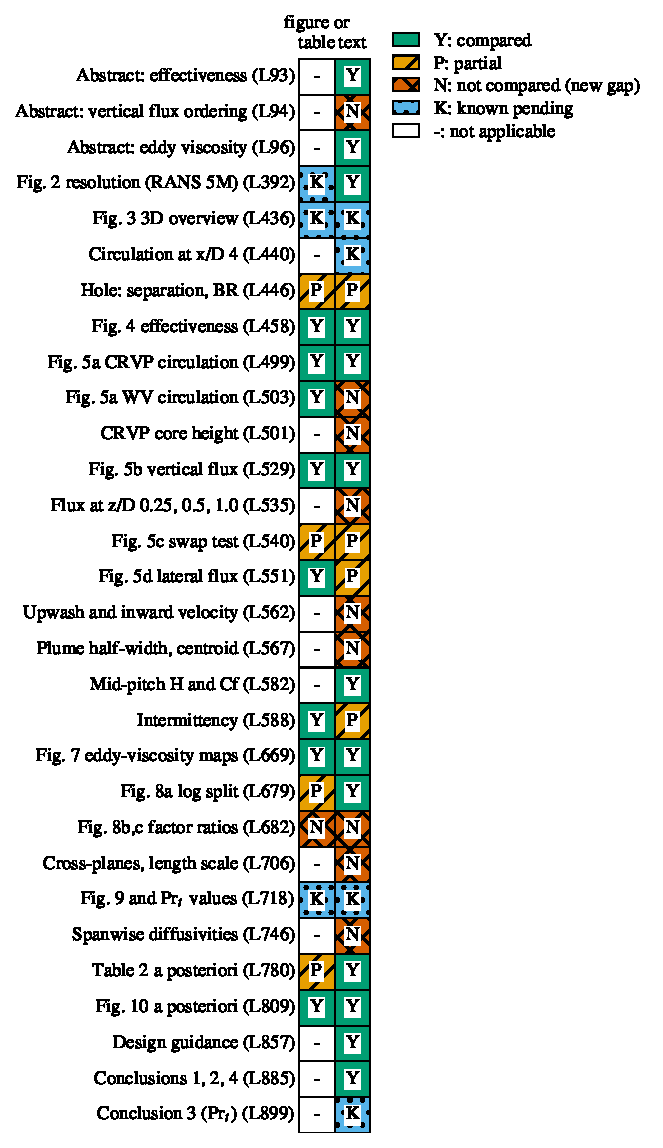
\includegraphics{ladder_grid.pdf}
\caption{Coverage of the 20M LES at each RANS--193M comparison. Y compared, P partial, N not compared, K known
pending, -- not applicable.}\label{fig:ladder}
\end{figure}

{\small
\begin{longtable}{@{}L{4.2cm} l l l L{7.0cm}@{}}
\toprule
Place & L & Fig./Tab. & Text & Note \\
\midrule
\endhead
Abstract, $\etab$ & 93 & -- & Y & \\
Abstract, vertical flux ordering & 94 & -- & N & LES crosses at $x/D=4.0$; not in the abstract \\
Abstract, eddy viscosity & 96 & -- & Y & \\
Fig.~2 resolution & 392 & K & Y & 20M mesh drawn; RANS 5M pending \\
Fig.~3 overview & 436 & K & K & known pending \\
Circulation at $x/D=4$ & 440 & -- & K & volume definition available (item 7) \\
Hole, separation and $\BR$ & 446 & P & P & LES $\BR$ in Table 1 only \\
Fig.~4 effectiveness & 458 & Y & Y & \\
Fig.~5a CRVP & 499 & Y & Y & no LES plane at 4, 10 \\
Fig.~5a WV & 503 & Y & N & 0.70--1.17 of the reference, not stated \\
CRVP core height & 501 & -- & N & \\
Fig.~5b vertical flux & 529 & Y & Y & mean-flow range incomplete (2.1) \\
Flux at $z/D$ 0.25, 0.5, 1.0 & 535 & -- & N & \\
Fig.~5c swap & 540 & P & P & LES total only; swap data for the LES exist \\
Fig.~5d lateral & 551 & Y & P & selected stations (2.2) \\
Upwash, inward velocity & 562 & -- & N & \\
Plume half-width, centroid & 567 & -- & N & \\
Mid-pitch $H$, $C_f$ & 582 & -- & Y & ``scale-resolving simulations'' \\
Intermittency & 588 & Y & P & plane mean RANS and 193M only \\
Fig.~7 maps & 669 & Y & Y & \\
Fig.~8a log split & 679 & P & Y & LES total only \\
Fig.~8b,c factors & 682 & N & N & \\
Cross-planes, length & 706 & -- & N & \\
Fig.~9, $\Pr_t$ & 718 & K & K & known pending \\
Spanwise diffusivities & 746 & -- & N & \\
Table 2 & 780 & P & Y & LES recovered share blank (2.9) \\
Fig.~10 & 809 & Y & Y & \\
Design guidance & 857 & -- & Y & wording (1.4) \\
Conclusions 1, 2, 4 & 885 & -- & Y & \\
Conclusion 3, $\Pr_t$ & 899 & -- & K & \\
\bottomrule
\end{longtable}}

%=====================================================================================================
\section{Figure and table check (item 3)}\label{sec:figtable}

Printed size from the stand-in class (textwidth 7.5\,in, columnwidth 3.56\,in). ``Ref/float'' gives the page of
the first text reference and of the float.

{\small
\begin{longtable}{@{}l >{\raggedright\arraybackslash\scriptsize}p{3.2cm} L{2.3cm} L{1.7cm} L{2.3cm} L{2.6cm} L{2.0cm}@{}}
\toprule
No. & File & Caption vs drawing & Ref/float & Style, LES & Text size, cmap, title & Verdict \\
\midrule
\endhead
Fig.~1 & \texttt{fig\_config\_regions.pdf} & matches & p3/p4 & n/a & 10\,pt; none; no title & OK \\
Fig.~2 & \texttt{fig\_resolution.pdf} & matches; panel (b) pooled to 25 (pending) & p4/p4 & 20M orange dash-dot &
10\,pt; none; no title & FINDING 3.8 \\
Fig.~3 & \texttt{fig\_overview\_3d.png} & matches; no LES (pending) & p6/p5 & n/a & 10\,pt; \texttt{jet} for
$\eta$, \texttt{bwr} for $\omega_x$; no title & FINDING 3.9 \\
Fig.~4 & \texttt{fig\_eta\_x.pdf} & band not in caption & p6/p6 & LES orange dash-dot; RANS 50M green & 10\,pt;
none; no title & FINDING 3.1, 3.7 \\
Fig.~5 & \texttt{fig\_coolant\_budget.pdf} & matches; $J_w$, $J_y$ undefined & p6/p7; cited before Fig.~4 & LES
orange solid/dashed; RANS blue & 10\,pt; none; no title & FINDING 3.2, 3.3, 3.5 \\
Fig.~6 & \texttt{fig\_spots.png} & matches & p9/p8 & n/a & 10\,pt; \texttt{inferno}; no title & OK \\
Fig.~7 & \texttt{fig\_meff\_maps.png} & matches & p9/p10 & n/a & 10\,pt; \texttt{bwr} symmetric in log; no title &
OK (3.11 optional) \\
Fig.~8 & \texttt{fig\_meff\_split\_film.pdf} & matches & p9/p10 & LES orange dash-dot; RANS total black & 10\,pt;
none; no title & FINDING 3.6 \\
Fig.~9 & \texttt{fig\_prt\_classic\_span.png} & matches & p11/p12 & n/a & 10\,pt; \texttt{inferno}; no title & OK
\\
Fig.~10 & \texttt{fig\_aposteriori.pdf} & matches; styles named in text & p11/p13 & LES orange dash-dot; base
blue & 10\,pt; none; no title & FINDING 3.1, 3.4 \\
Tab.~1 & (in source) & matches & p3/p4 & -- & -- & OPEN L309 \\
Tab.~2 & (in source) & matches & p11/p12 & LES row present & -- & FINDING 2.9 (optional) \\
\bottomrule
\end{longtable}}

Every figure is referenced; first references follow the order 1, 2, 3, 5, 4, 6, 7, 8, 9, 10 (finding 3.3).

\end{document}
